\documentclass{article}
\usepackage{graphicx}
\usepackage{float}
\usepackage{multirow}
\usepackage{booktabs}

\begin{document}
\title{Graphs for hw3}
\author{Jinhui Zhang}
\date{\today}

\maketitle
The numbers of test samples I used are through 1 to 20 except 17. 

\section{Uninformed search}
\begin{figure}[h]
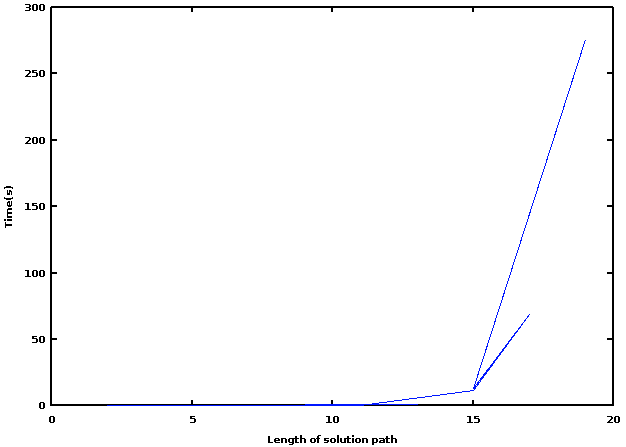
\includegraphics[width=1.0\textwidth]{uninformed.png}
\caption{The time cost(s) and the length of solution path in uniformed search}
\end{figure}
Experimental result shows below. 
\begin{table}[H]
\caption{Experimental results of uninformed search}
    \begin{tabular}{ccc}
    \toprule
    Problem number & Length of solution path & Time(s)               \\
    \midrule
    1         & 6                       & 0.001956939697265625  \\
    2         & 4                       & 0.0004558563232421875 \\
    3         & 2                       & 5.602836608886719e-05 \\
    4         & 6                       & 0.0015571117401123047 \\
    5         & 4                       & 0.0004520416259765625 \\
    6         & 9                       & 0.03304100036621094   \\
    7         & 3                       & 0.00014495849609375   \\
    8         & 5                       & 0.0005011558532714844 \\
    9         & 5                       & 0.0007290840148925781 \\
    10        & 5                       & 0.001007080078125     \\
    11        & 9                       & 0.02097797393798828   \\
    12        & 9                       & 0.06315898895263672   \\
    13        & 13                      & 0.9659819602966309    \\
    14        & 5                       & 0.0010759830474853516 \\
    15        & 11                      & 0.19655299186706543   \\
    16        & 15                      & 11.44983696937561     \\
    18        & 17                      & 68.86690998077393     \\
    19        & 15                      & 13.28905200958252     \\
    20        & 19                      & 276.18528294563293    \\
    \bottomrule
    \end{tabular}
\end{table}

\section{Informed search(h1)}
The h1 function is the number of misplaced tiles. 
\begin{figure}[H]
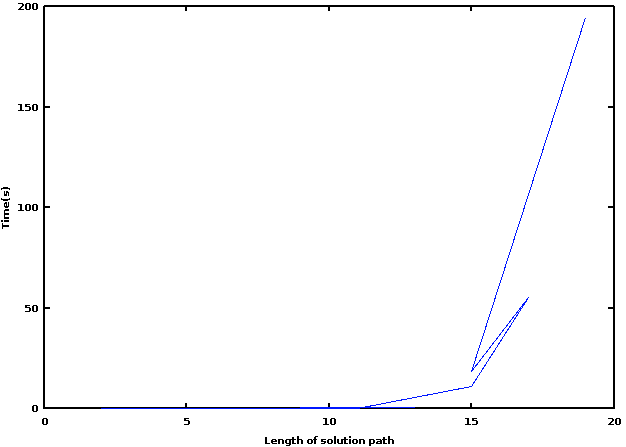
\includegraphics[width=1.0\textwidth]{h1.png}
\caption{The time cost(s) and the length of solution path in informed search with heuristic function h1}
\end{figure}
Experimental result shows below. 
\begin{table}[H]
\caption{Experimental results of informed search(h1)}
    \begin{tabular}{ccc}
    \toprule
    Problem number & Length of solution path & Time(s)               \\
    \midrule
    1         & 6                       & 0.00025010108947753906  \\
    2         & 4                       & 0.0001709461212158203 \\
    3         & 2                       & 5.698204040527344e-05 \\
    4         & 6                       & 0.0002620220184326172 \\
    5         & 4                       & 0.0002009868621826172 \\
    6         & 9                       & 0.02200007438659668   \\
    7         & 3                       & 9.989738464355469e-05   \\
    8         & 5                       & 0.0002110004425048828 \\
    9         & 5                       & 0.0002701282501220703 \\
    10        & 5                       & 0.00019097328186035156     \\
    11        & 9                       & 0.016025066375732422   \\
    12        & 9                       & 0.04271197319030762   \\
    13        & 13                      & 0.7884721755981445    \\
    14        & 5                       & 0.0002219676971435547 \\
    15        & 11                      & 0.11528301239013672   \\
    16        & 15                      & 11.352113962173462     \\
    18        & 17                      & 55.4756019115448     \\
    19        & 15                      & 18.732638120651245     \\
    20        & 19                      & 194.611093044281    \\
    \bottomrule
    \end{tabular}
\end{table}


\section{Informed search(h2)}
The h2 function is written by my own, that is the subtractions of the tiles in current state and the tiles in goal state. It still needs improvement in performance. 
\begin{figure}[H]
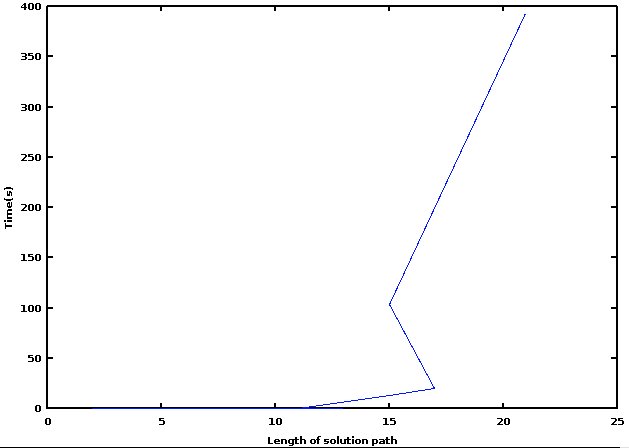
\includegraphics[width=1.0\textwidth]{h2.png}
\caption{The time cost(s) and the length of solution path in informed search with heuristic function h2}
\end{figure}
Experimental result shows below. 
\begin{table}[H]
\caption{Experimental results of informed search(h2)}
    \begin{tabular}{ccc}
    \toprule
    Problem number & Length of solution path & Time(s)               \\
    \midrule
    1         & 6                       & 0.0002880096435546875  \\
    2         & 4                       & 0.000347137451171875 \\
    3         & 2                       & 0.00010013580322265625 \\
    4         & 6                       & 0.0006811618804931641 \\
    5         & 4                       & 0.0004029273986816406 \\
    6         & 9                       & 0.0008001327514648438   \\
    7         & 3                       & 0.00018405914306640625   \\
    8         & 5                       & 0.00027298927307128906 \\
    9         & 5                       & 0.0003020763397216797 \\
    10        & 5                       & 0.0003871917724609375    \\
    11        & 9                       & 0.0006659030914306641   \\
    12        & 9                       & 0.0007989406585693359    \\
    13        & 13                      & 0.005901813507080078    \\
    14        & 5                       & 0.0005559921264648438 \\
    15        & 11                      & 0.5104520320892334   \\
    16        & 15                      & 13.110538005828857     \\
    18        & 17                      & 20.030537843704224     \\
    19        & 15                      & 104.06644606590271     \\
    20        & 19                      & 392.7996838092804    \\
    \bottomrule
    \end{tabular}
\end{table}
\end{document}
